% \begin{table}[!htb]
%   \caption{\textit{Continuação} - Práticas identificadas no pensamento computacional, segundo \citeonline{Barr2011}, presentes/possíveis na educação básica}
%   \label{tab:facetas}
%   \begin{center}
%     \begin{tabularx}{\textwidth}{@{}YYYYYY@{}}
%       \hline 
      
%       \textbf{Práticas} & \textbf{Matemática} & \textbf{Ciências} & \textbf{Estudos Sociais} & \textbf{Linguagens} \\

%       \hline
%       \\
%       \textit{Procedimentos algorítmicos} & Longa divisão, fatoração & Fazer procedimentos experimentais & - & Escrever instruções \\ \\ % 

%       \hline
%       \\
%       \textit{Automação} & - & Usar \textit{Probware} ou \textit{Origin} & Usar excel & Usar um corretor ortográfico \\ \\ 

%       \hline
%       \\
%       \textit{Paralelização} & Resolver sistema lineares; fazer multiplicação de matrizes & Executar simultaneamente experimentos com diferentes parâmetros & - & - \\ \\

%       \hline
%       \\
%       \textit{Simulação} & Representar graficamente uma função em um plano cartesiano e modificar os valores da variáveis & Simular o movimento de o sistema solar & Jogar Age of Empires; Trilha de Oregon & Fazer uma reencenação de uma história \\ \\
%       \hline

%     \end{tabularx}
%   \end{center}
%   \legend{Fonte: Adaptado de \citeonline{Barr2011}}
% \end{table}

% \begin{table}[htbp]
%   %  \centering does nothing if table is full width
%     \caption{Add caption}
%       \begin{tabularx}{\textwidth}{@{}YYYYYY@{}}
%       % \begin{tabularx}{\textwidth}{*{3}{>{\centering\arraybackslash}X}}
%       \toprule
%       \textbf{Aditivo} & \multicolumn{2}{c}{\textbf{Quantidade (g)}}\\
%       \cmidrule{2-3}
%        & \multicolumn{2}{c}{Carga Mineral (\%)} \\
%        & 20    & 30 \\
%        \midrule
%       \multirow{3}{*}{Fibra} & 1,266 & 252 \\
%       % GCC & 0,316 & 52 \\
%       % Amido & 0,016 & 25 \\
%       % ASA & 0,002 & 252 \\
%       % Percol & 0,00032 & 25 \\
%       \bottomrule
%       \end{tabularx}
%     \label{tab_formacao_folhas}%
%   \end{table}

%   \begin{tabular}{|l|l|l|l|}\hline
%     \multirow{10}{*}{numeric literals} & \multirow{5}{*}{integers} & in decimal & \verb|8743| \\ 
%     & & \multirow{2}{*}{in octal} & \verb|0o7464| \\ 
%     & & & \verb|0O103| \\ 
%     & & \multirow{2}{*}{in hexadecimal} & \verb|0x5A0FF| \\ 
%     & & & \verb|0xE0F2| \\ 
%     & \multirow{5}{*}{fractionals} & \multirow{5}{*}{in decimal} & \verb|140.58| \\ 
%     & & & \verb|8.04e7| \\ 
%     & & & \verb|0.347E+12| \\ 
%     & & & \verb|5.47E-12| \\ 
%     & & & \verb|47e22| \\ 
%     \multicolumn{3}{|l|}{\multirow{3}{*}{char literals}} & \verb|'H'| \\ 
%     \multicolumn{3}{|l|}{} & \verb|'\n'| \\ 
%     \multicolumn{3}{|l|}{} & \verb|'\x65'| \\ 
%     \multicolumn{3}{|l|}{\multirow{2}{*}{string literals}} & \verb|"bom dia"| \\ 
%     \multicolumn{3}{|l|}{} & \verb|"ouro preto\nmg"| \\ 
%   \end{tabular}
  
  \begin{tabular}{|l|l|l|l|}\hline
    \multirow{10}{*}{numeric literals} & \multirow{5}{*}{integers} & in decimal & \verb|8743| \\ 
    && \multirow{2}{*}{in octal} & \verb|0o7464| \\ 
    & & & \verb|0O103| \\ 
    & & \multirow{2}{*}{in hexadecimal} & \verb|0x5A0FF| \\ 
    & & & \verb|0xE0F2| \\ 
    & \multirow{5}{*}{fractionals} & \multirow{5}{*}{in decimal} & \verb|140.58| \\ 
    & & & \verb|8.04e7| \\ 
    & & & \verb|0.347E+12| \\ 
    & & & \verb|5.47E-12| \\ 
    & & & \verb|47e22| \\ 
    & \multicolumn{2}{l|}{\raisebox{-\totalheight}{ 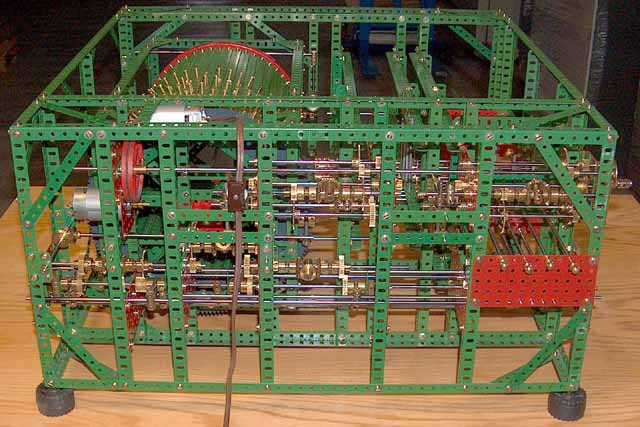
\includegraphics[width=0.3\textwidth]{imagens/babbage.jpg}} 
      } & \\  &\multicolumn{2}{p{4cm}|}{assim caminha toda a a ordem de ideais que rodopiam o mundo}  & \\ 

    % \raisebox{-\totalheight}{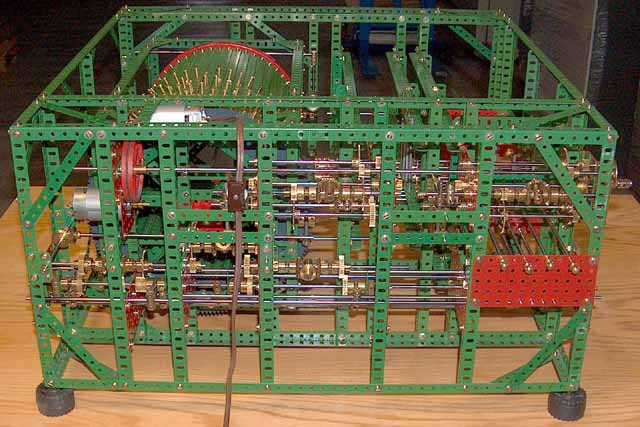
\includegraphics[width=0.3\textwidth, height=60mm]{imagens/babbage.jpg}}\\\\

    % \mutirow{4}{*}{
    % } \\ 
  \end{tabular}
  
\begin{landscape}
  
\begin{center}
 \begin{tabular}{L{6cm}L{6cm}L{5cm}L{5cm}}
    \hline
    Atividade & Faceta & Prática Envolvida & Classificação taxonômica da prática \\
    \hline
    \multirow{3}{*}{\shortstack[l]{Projeto de construtor de\\ montanha-russa\\ \includegraphics{}}} & Os alunos constroem modelos de montanhas-russas que podem ser executadas, gerando dados sobre a energia da montanha-russa  & Obter insight / compreensão de simulações / modelos baseados em computador & Uso de um modelo computacional para entender um conceito \\ 
    && \multirow{3}{*}{\shortstack[l]{in\\ octal\\ 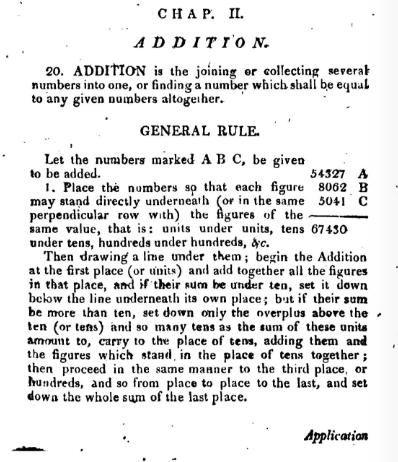
\includegraphics[width=0.03\textwidth]{imagens/algorithm.png}}} & \verb|0o7464| \\ 
    & & & \verb|0O103| \\ 
    & & \multirow{2}{*}{in hexadecimal} & \verb|0x5A0FF| \\ 
    & & & \verb|0xE0F2| \\ 
    & \multirow{5}{*}{fractionals} & \multirow{5}{*}{in decimal} & \verb|140.58| \\ 
    & & & \verb|8.04e7| \\ 
    & & & \verb|0.347E+12| \\ 
    & & & \verb|5.47E-12| \\ 
    & & & \verb|47e22| \\ 
    & \multicolumn{2}{l}{\raisebox{-\totalheight}{ 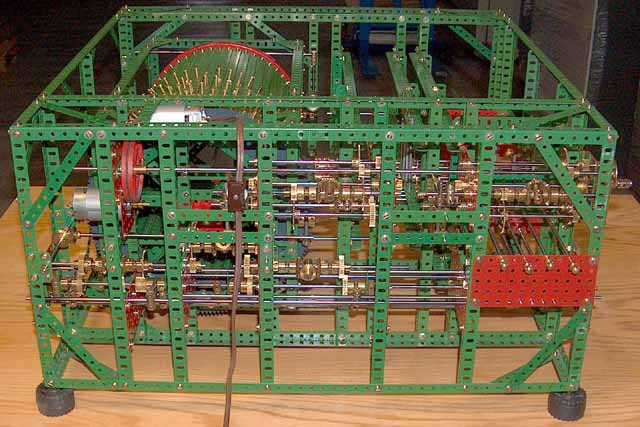
\includegraphics[width=0.3\textwidth]{imagens/babbage.jpg}} 
      } & \\  &\multicolumn{2}{p{4cm}}{assim caminha toda a a ordem de ideais que rodopiam o mundo}  & \\ 

    % \raisebox{-\totalheight}{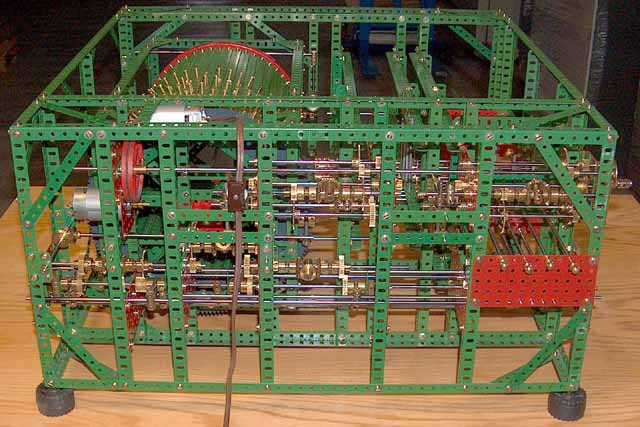
\includegraphics[width=0.3\textwidth, height=60mm]{imagens/babbage.jpg}}\\\\

    % \mutirow{4}{*}{
    % } \\ 
  \end{tabular}
\end{center}
\end{landscape}
